\chapter{Musterlösung}

Alle Wireshark Mitschnitte liegen als \grqq *.pcapng \grqq{} Datei bei.

\subsection{Aufgabe 2.1 - Joining einer Phillips Hue Lampe}

\begin{figure}[H]
    \centering
    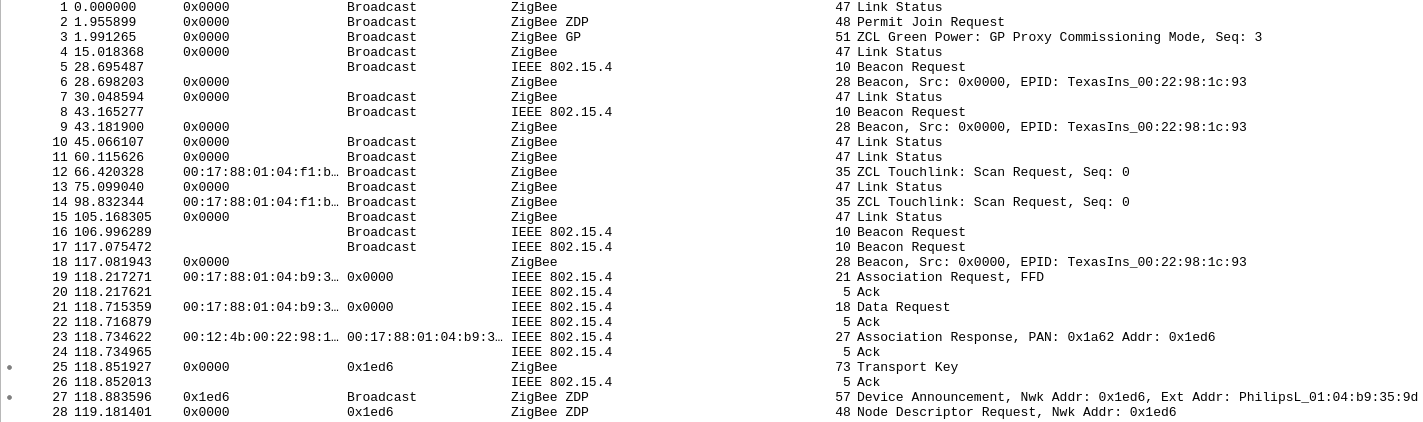
\includegraphics[width=1\textwidth]{media/lsg2.1-1.png}
    \caption{Wireshark Ausschnitt - Joining einer Lampe Teil 1}
\end{figure}

Im ersten Teil ist der Physikalische Verbindungsaufbau zu sehen. Mit Paket 2 erlaubt der Koordinator
allen Mitgliegern die Aufnahme weiterer Geräte. Paket 5 ist ein Beacon der Lampe, welcher den Beitrittswunsch
signalisiert. Auf diesen Antwortet der Koordinator jeweils mit einem Beacon Response. Nun folgt ein Association
Request sowie Data Request der Lampe (19). In der Association Response (23) bekommt die Lampe
Ihre kurze Adresse zugewiesen. In Paket 25 wird der Transport Key zur verschlüsselten Kommunikation 
übermittelt.

\begin{figure}[H]
    \centering
    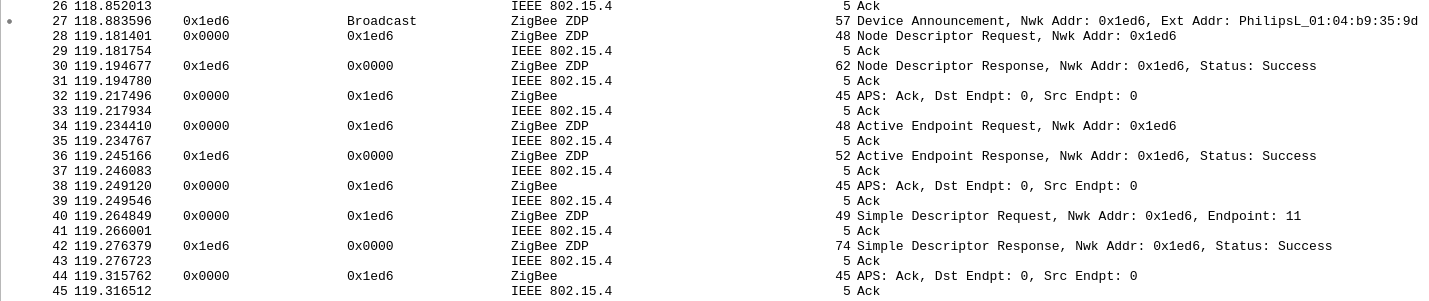
\includegraphics[width=1\textwidth]{media/lsg2.1-2.png}
    \caption{Wireshark Ausschnitt - Joining einer Lampe Teil 2}
\end{figure}

Im Anschluss fragen die Geräte gegenseitig ihre Aktiven Endpunkte über \grqq Node Descriptor\grqq{} Nachrichten ab. Die einzelnen Endpunkte werden im Anschluss per \grqq 
Active Endpoint Requests\grqq{} interviewed und per \grqq Simple Descriptor\grqq{} Nachrichten beschrieben.

\subsection{Aufgabe 2.2 - Schalten einer Lampe}

\begin{figure}[H]
    \centering
    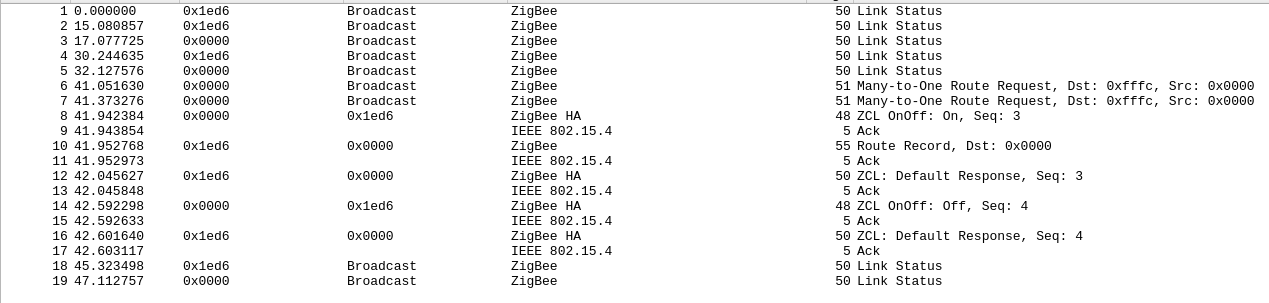
\includegraphics[width=1\textwidth]{media/lsg2.2.png}
    \caption{Wireshark Ausschnitt - Schalten einer Lampe}
\end{figure}

Hier ein ein Ein- und Auschaltvorgang einer Lampe zu sehen. Zum Schalten wird jeweils ein \grqq ZigBee Kommando Frame\grqq{} versendet, welches erst Physikalisch und 
anschließend auf ZigBee Ebene bestätigt wird.

\subsection{Aufgabe 3 - Joining einer Fernbedienung über die Lampe}

\begin{figure}[H]
    \centering
    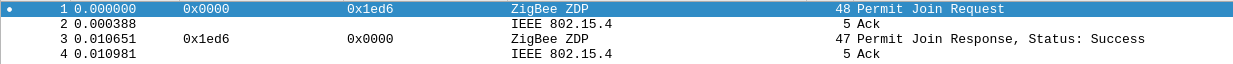
\includegraphics[width=1\textwidth]{media/lsg-3-1.png}
    \caption{Wireshark Ausschnitt - Schalten einer Lampe}
\end{figure}

Hier erteilt der Koordinator der Lampe die Erlaubniss neue Geräte in das Netzwerk aufzunehmen.

\begin{figure}[H]
    \centering
    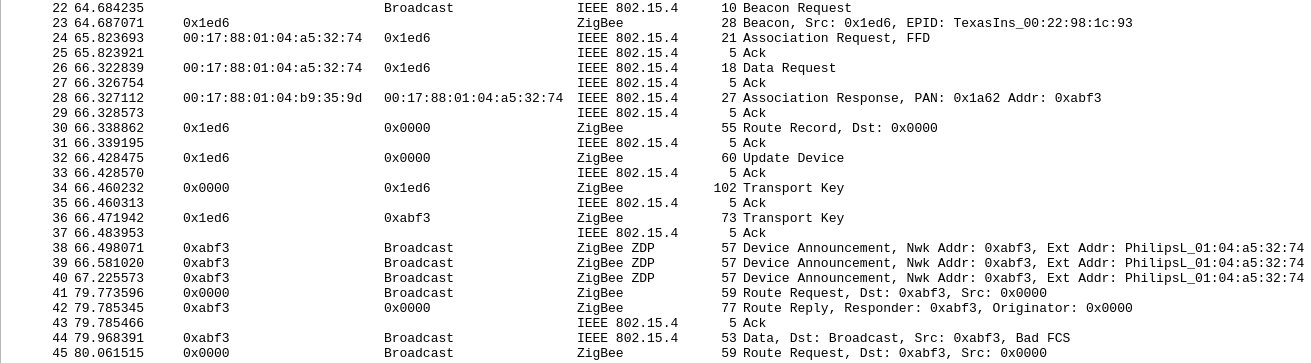
\includegraphics[width=1\textwidth]{media/lsg-3-2.png}
    \caption{Wireshark Ausschnitt - Schalten einer Lampe 1}
\end{figure}

Die hat zur Folge, dass die Lampe auf die Beacon-Requests der Lampe mit Beitrittswunsch reagiert. Diese Beacons dienen dazu, das Netzwerk der neuen Lampe bekannt zu machen.
Mit Nachricht 24 erfragt die neue Lampe einen Beitritt in das Netzwerk. Der Lampe wird eine Kurze Adresse sowie die PAN-ID von der Lampe im Netzwerk zugewiesen. Anschließend 
macht die bestehende Lampe das neue Gerät dem Koordinator bekannt. Dieser versendet im Anschluss den Netzwerk Schlüssel. Dieser wird in einem Tunnel verschlüsselt bis zu dem letzten
Gerät vor dem neuen Teilnehmer übermittelt. Im Anschluss erfolgt das Interview des neuen Gerätes, dies ist identisch zu Aufgabe 2.

\subsection{Aufgabe 4 - Binding der Fernbedienung}

\begin{figure}[H]
    \centering
    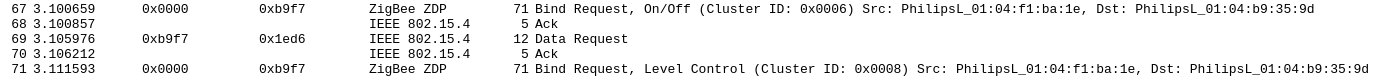
\includegraphics[width=1\textwidth]{media/lsg-4-1.png}
    \caption{Wireshark Ausschnitt - Binden einer Lampe 1}
\end{figure}

Die Bindung wird durch ein Bind-Request von dem Koordinator an die Fernbedienung initiiert. Hier Paket 67 und 71.

\begin{figure}[H]
    \centering
    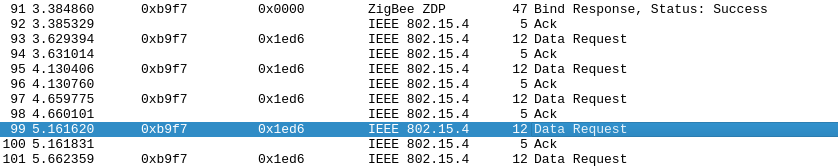
\includegraphics[width=1\textwidth]{media/lsg-4-2.png}
    \caption{Wireshark Ausschnitt - Binden einer Lampe 2}
\end{figure}

Die Fernbedienung bestätigt eine erfolgreiche Bindung durch eine Bind-Response Nachricht mit einem \grqq Success\grqq{} im Payload.
Im Anschluss beginnt die Fernbedienung mit Polling, um zu überprüfen ob weitere Nachrichten für sie verfügbar sind.

\begin{figure}[H]
    \centering
    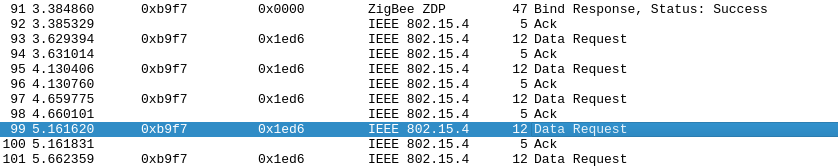
\includegraphics[width=1\textwidth]{media/lsg-4-2.png}
    \caption{Wireshark Ausschnitt - Schalten einer Lampe mit Binding}
\end{figure}

Die ZCL Nachricht wird nun direkt von der Fernbedienung an die Lampe als Unicast geschickt.

\subsection{Aufgabe 5 - Gruppenbildung}

\begin{figure}[H]
    \centering
    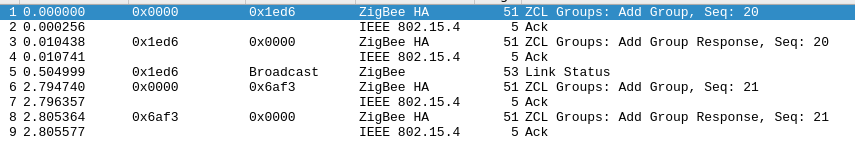
\includegraphics[width=1\textwidth]{media/lsg-5-1.png}
    \caption{Wireshark Ausschnitt - Schalten einer Lampe mit Binding}
\end{figure}

Zuerst wird die Gruppe angelegt. Dafür wird an die jeweiligen Geräte eine Add Group Nachricht gesendet. Diese wird mit einer jeweiligen Respone
Nachricht bestätigt.

\begin{figure}[H]
    \centering
    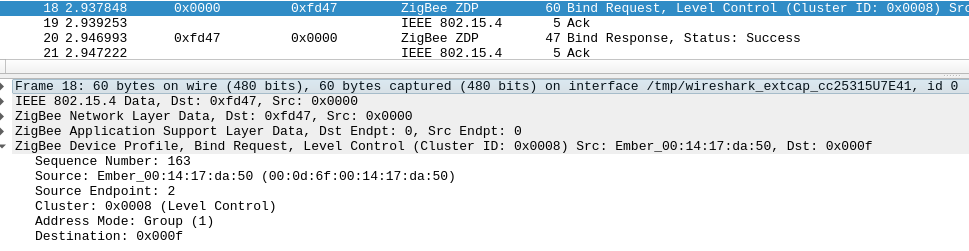
\includegraphics[width=1\textwidth]{media/lsg-5-2.png}
    \caption{Wireshark Ausschnitt - Schalten einer Lampe mit Binding}
\end{figure}

Im Anschluss wird die Gruppe an den Endpunkt der Fernbedienung gebunden. Der Fernbedienung wird diesmal als Ziel die Gruppen Broadcast Adresse
0x000F sowie der Adressmodus Gruppe mitgeteilt. Auch dies wird von der Fernbedienung wieder bestätigt. Das Reporting welches im Anschluss 
konfiguriert wird ist eine Eigenart von zigbee2mqtt. Damit wird der Koordinator um Zustandsänderungen der Lampe informiert, um diese Informationen
beispielweiße an eine zentrale Heimautomatisierung weiterzugeben.

Beim Schalten wird das ZCL Kommando nun an die Gruppenadresse 0x000F versendet. Die zu schaltenden Geräte überprüfen selbst ob sie in der Gruppe sind 
oder nicht. Prinzipiell erhällt jedes Gerät im Netzwerk das Kommando.

\subsection{Fragen}
\subsubsection{Aufgabe 2}




